
\documentclass[fleqn,addpoints]{exam}

\usepackage{units} 
\usepackage{graphicx}
\usepackage[fleqn]{amsmath}
\usepackage{cancel}
\usepackage{float}
\usepackage{mdwlist}
\usepackage{booktabs}
\usepackage{cancel}
\usepackage{polynom}
\usepackage{caption}
\usepackage{fullpage}
\usepackage{xfrac}
\usepackage{enumerate}

\everymath{\displaystyle}

% \printanswers

\ifprintanswers
  \usepackage{2in1, lscape}
\fi

\title{Math 141 Chapter Four Exam}
\date{July 17, 2013}
\author{}

\begin{document}

  \maketitle  

  % \vspace{0.2in}
  % \makebox[\textwidth]{Name:\enspace\hrulefill}
  % \vspace{0.2in}

  \begin{center}
  \gradetable[h][pages]
  \bonusgradetable[h][pages]
  \end{center}

  \begin{questions}
    \uplevel{\section{Questions}}

    \question Write in logarithm form
      \begin{parts}
        \part[2] $2^3 = 8$

        \part[2] $e^x = y$
      \end{parts}

    \question Write in exponential form
      \begin{parts}
        \part[2] $\log_3 81 = 4$

        \part[2] $\ln x = 5$
      \end{parts}

    \question Evaluate each expression.
      \begin{parts}

        \part[2] $\log_8 64$

        \part[2] $\log 0.001$

        \part[2] $\log_7 \frac{1}{49}$

        \part[2] $\log_9 27$

        \part[2] $\log_8 16 + \log_8 32$

        \part[2] $\log_5 100 - \log_5 4$

      \end{parts}

    \question[5] solve for x:
      \[
        \log_x 27 = \frac{3}{2}
      \]

    \question Write as the sum/difference of logarithms:
      \begin{parts}
        \part[5]
          \[
            \log \left( \frac{x^2y^3}{z} \right)
          \]

        \part[7]
          \[
            \log_5 \sqrt{ \frac{2x^3}{(x + 1)^3 (x - 2)^2} }
          \]

        \part[7]
          \[
            \ln \left[ \frac{ \sqrt{x + 2} \sqrt[3]{x - 1} }{ (x + 3)^4 } \right]
          \]

      \end{parts}

    \question[7] Write as a single logarithm:
      \begin{parts}
        \part[5] $\log x + 2 \log(x - 1)$

        \part[7] $\ln (x + 2) + 2 \ln (x + 3) - \frac{1}{2} \ln x$

        \part[7] $\log \sqrt{x - 1} + \log{x + 1} - 2 \log\left( x^2 + 1 \right)$

      \end{parts}

      \begin{solution}
        \begin{align*}
          \ln (x + 2) + 2 \ln (x + 3) - \frac{1}{2} \ln x & = \ln (x + 2) + \ln (x + 3)^2 - \ln x^{1/2} \\
                                                          & = \ln \left[ (x + 2)(x + 3)^2 \right] - \sqrt{x} \\
                                                          & = \ln \frac{ (x + 2)(x + 3)^2 }{\sqrt{x}} \\
        \end{align*}
      \end{solution}

    \question[3] Write as a combination of base 10 logarithms: $\log_5 7$ 

    \question Solve for $x$
      \begin{parts}
        \part[7] $e^{2x} x^2 - 2 e^{2x} x - 5 e^{2x} = 0$
          \begin{solution}
            \begin{align*}
              e^{2x} x^2 - 2 e^{2x} x - 5 e^{2x} & = 0 \\
              e^{2x} \left( x^2 - 2x - 5 \right) & = 0 \\
              \\
              x                                  & = \frac{2 \pm \sqrt{4 - 4 (-5)}}{2} \\
                                                 & = \frac{2 \pm \sqrt{24}}{2} \\
                                                 & = \frac{2 \pm 2 \sqrt{6}}{2} \\
                                                 & = 1 \pm \sqrt{6} \\
            \end{align*}
          \end{solution}

        \part[7] $2e^{2x} - 7e^x - 4 = 0$
          \begin{solution}
            \begin{align*}
              2e^{2x} - 7e^x - 4                               & = 0 \\
              \left( 2e^x + 1 \right) \left( e^x - 4 \right) & = 0 \\
              x                                              & = \boxed{ \ln 4 } \\
            \end{align*}
          \end{solution}

          \part[7] $3^{2x} = 4^{x - 1}$
          \begin{solution}
            \begin{align*}
              3^{2x}              & = 4^{x - 1} \\
              \ln 3^{2x}          & = \ln 4^{x - 1} \\
              2x \ln 3            & = (x - 1) \ln 4 \\
              2x \ln 3            & = x \ln 4 - \ln 4 \\
              x \ln 4 - 2x \ln 3  & =  \ln 4 \\
              x (\ln 4 - 2 \ln 3) & =  \ln 4 \\
              x                   & = \frac{\ln 4}{\ln 4 - 2 \ln 3} \\
            \end{align*}
          \end{solution}
          
          \part[7] $\log_2(3x - 1) - \log_2(x - 1) = \log_2(x + 1)$
          \begin{solution}
            \begin{align*}
              \log_2(8x - 1) - \log_2(x - 1)             & = \log_2(x + 1) \\
              \log_2 \left( \frac{8x - 1}{x - 1} \right) & = \log_2(x + 1) \\
              \frac{8x - 1}{x - 1}                       & = x + 1 \\
              8x - 1                                     & = x^2 - 1 \\
              x^2 - 8x                                   & = 0 \\
              x(x - 8)                                   & = 0 \\
              x                                          & = 8 \\
            \end{align*}
          \end{solution}
      \end{parts}

    \question[7]
      If you deposit \$1,000 in an account earning 12\% interest compounded monthly, how long will it take for the money
      to double?

      \begin{solution}
        \begin{align*}
          2000  & = 1000 \left( 1 + \frac{0.12}{12} \right)^{12t} \\
          2     & = ( 1 + 0.01 )^{12t} \\
          \ln 2 & = \ln (1.01)^{12t} \\
          \ln 2 & = 12 t \ln 1.01 \\
          t     & = \frac{\ln 2}{12 \ln 1.01 } \\
                & \approx \unit[5.8]{year} \\
        \end{align*}
      \end{solution}

    \question[10]
      If Carbon 14 has a half-life of 5,730 years and 80\% of the original Carbon 14 in a sample has decayed into Carbon
      12, how old is the sample?

      \begin{solution}
        find the rate:
        \begin{align*}
          0.5 m_0 & = m_0 e^{-5730r} \\
          \ln 0.5 & = -5730r \\
          - \ln 2 & = -5730r \\
          r       & = \frac{\ln 2}{5730} \\
                  & \approx 0.0001210 \\
        \end{align*}

        find the age:
        \begin{align*}
          0.2 m_0 & = m_0 e^{-0.0001210 t} \\
          0.2     & = e^{-0.0001210 t} \\
          \ln 0.2 & = -0.0001210 t \\
          t       & = \frac{\ln 0.2}{-0.0001210} \\
                  & \approx \unit[13,305]{years} \\
        \end{align*}
      \end{solution}

    \question[7]
      If the magnitude of a sound is 85 dB, what is its intensity?  
      
      % If the intensity of the crowd sound at a Seahawks game is $I = \unit[1 \times 10^{-5}]{W/m^2}$, what is the
      % magnitude of the sound in decibels?

      \begin{solution}
        \begin{align*}
          M        & = 10 \log \frac{I}{I_0} \\
          \\
          85       & = 10 \log \frac{I}{10^{-12}} \\
          8.5      & = \log \frac{I}{10^{-12}} \\
          10^{8.5} & = \frac{I}{10^{-12}} \\
          I        & = 10^{-3.5} \\
        \end{align*}
      \end{solution}

    \question $f(x) = 1 - 2^{-x}$
      \begin{parts}
        \part[2] what is the domain?

        \part[2] what is the range?

        \part[2] what is the y-intercept?

        \part[5] plot the graph
          \begin{solution}
            \begin{figure}[H]
              \centering
              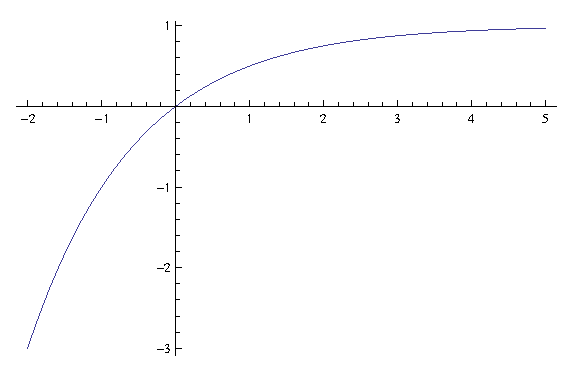
\includegraphics[scale=0.9]{graph_1.eps}
              \caption*{$f(x) = 1 - 2^x$}
            \end{figure}
          \end{solution}

      \end{parts}

    \question $f(x) = \log_2 (x - 1)$
      \begin{parts}
        \part[2] what is the domain?

        \part[2] what is the range?

        \part[2] what is the y-intercept?

        \part[5] plot the graph
          \begin{solution}
            \begin{figure}[H]
              \centering
              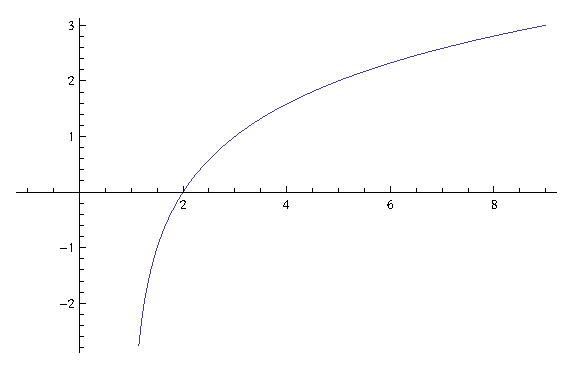
\includegraphics[scale=0.9]{graph_2.eps}
              \caption*{ $f(x) = \log_2 (x - 1)$ }
            \end{figure}
          \end{solution}
      \end{parts}


    \uplevel{\section{Extra Credit}}

    \bonusquestion[10]
      \[
        f(x) = \frac{3}{1 + 2e^{-0.2x}} 
      \]

      Find $f^{-1}(x)$

      \begin{solution}

        solve for $x$ in terms of $y$:
        \begin{align*}
          y               & = \frac{3}{1 + 2e^{-0.2x}} \\
          y + 2ye^{-0.2x} & = 3 \\
          2ye^{-0.2x}     & = 3 - y \\
          e^{-0.2x}       & = \frac{3 - y}{2y} \\
          -0.2x           & = \ln \left( \frac{3 - y}{2y} \right) \\
          - \frac{x}{5}   & = \ln \left( \frac{3 - y}{2y} \right) \\
          x               & = -5 \ln \left( \frac{3 - y}{2y} \right) \\
        \end{align*}
        
        replace $y$ with $x$ to make a function of $x$:
        \[
          \boxed{ f^{-1}(x) = -5 \ln \left( \frac{3 - x}{2x} \right) } \\
        \]

      \end{solution}
  \end{questions}

\end{document}

